\documentclass{article} % For LaTeX2e
\usepackage{nips14submit_e,times}
\usepackage{amsmath}
\usepackage{amsthm}
\usepackage{amssymb}
\usepackage{mathtools}
\usepackage{hyperref}
\usepackage{url}
\usepackage{algorithm}
\usepackage[noend]{algpseudocode}
%\documentstyle[nips14submit_09,times,art10]{article} % For LaTeX 2.09

\usepackage{bbm}
\usepackage{graphicx}
\usepackage{caption}
\usepackage{subcaption}
\usepackage{MnSymbol}

\def\eQb#1\eQe{\begin{eqnarray*}#1\end{eqnarray*}}
\def\eQnb#1\eQne{\begin{eqnarray}#1\end{eqnarray}}
\providecommand{\e}[1]{\ensuremath{\times 10^{#1}}}
\providecommand{\pb}[0]{\pagebreak}
\DeclarePairedDelimiter\ceil{\lceil}{\rceil}
\DeclarePairedDelimiter\floor{\lfloor}{\rfloor}

\newcommand{\E}{\mathrm{E}}
\newcommand{\Var}{\mathrm{Var}}
\newcommand{\Cov}{\mathrm{Cov}}
\newcommand\eqD{\stackrel{\mathclap{\normalfont\mbox{d}}}{=}}

\def\Qb#1\Qe{\begin{question}#1\end{question}}
\def\Sb#1\Se{\begin{solution}#1\end{solution}}

\newenvironment{claim}[1]{\par\noindent\underline{Claim:}\space#1}{}
\newtheoremstyle{quest}{\topsep}{\topsep}{}{}{\bfseries}{}{ }{\thmname{#1}\thmnote{ #3}.}
\theoremstyle{quest}
\newtheorem*{definition}{Definition}
\newtheorem*{theorem}{Theorem}
\newtheorem*{lemma}{Lemma}
\newtheorem*{question}{Question}
\newtheorem*{preposition}{Preposition}
\newtheorem*{exercise}{Exercise}
\newtheorem*{challengeproblem}{Challenge Problem}
\newtheorem*{solution}{Solution}
\newtheorem*{remark}{Remark}
\usepackage{verbatimbox}
\usepackage{listings}
\usepackage{mathrsfs}
\title{ProbLimI: \\
Problem Set IX}


\author{
Youngduck Choi \\
CIMS \\
New York University\\
\texttt{yc1104@nyu.edu} \\
}


% The \author macro works with any number of authors. There are two commands
% used to separate the names and addresses of multiple authors: \And and \AND.
%
% Using \And between authors leaves it to \LaTeX{} to determine where to break
% the lines. Using \AND forces a linebreak at that point. So, if \LaTeX{}
% puts 3 of 4 authors names on the first line, and the last on the second
% line, try using \AND instead of \And before the third author name.

\newcommand{\fix}{\marginpar{FIX}}
\newcommand{\new}{\marginpar{NEW}}

\nipsfinalcopy % Uncomment for camera-ready version

\begin{document}


\maketitle

\begin{abstract}
This work contains solutions to the exercises of the problem set IX. The
chosen problems are 2,3 and 4.
\end{abstract}

\bigskip


\begin{question}[2]
\hfill
\begin{figure}[h!]
  \centering
    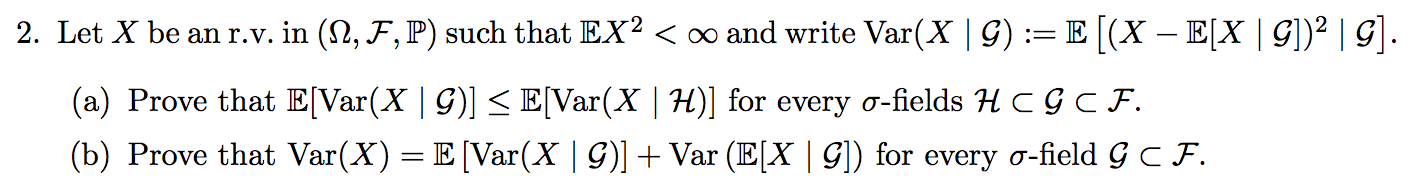
\includegraphics[width=0.7\textwidth]{problim-e9-p2.png}
\end{figure}
\end{question}
\begin{solution} \hfill \\
\textbf{(a)} The result intuitively makes sense, since on average
knowing more information should reduce variance. We compute
\eQnb
\mathbb{E}[\text{Var}(X|H)] &=& \mathbb{E}[(X - \mathbb{E}[X|H])^2]
= \mathbb{E}[(X - \mathbb{E}[X|G])^2]  + 
\mathbb{E}[(\mathbb{E}[X|G] - \mathbb{E}[X|H])^2] \nonumber \\
&+& 
2\mathbb{E}[(\mathbb{E}[X|G] - \mathbb{E}[X|H])(X - \mathbb{E}[X|G])] \nonumber \\
&=& \mathbb{E}[\text{Var}(X|G)] -  \mathbb{E}[(\mathbb{E}[X|G] - \mathbb{E}[X|H])^2] 
\geq \mathbb{E}[\text{Var}(X|G)] 
\label{eq:2.a} 
\eQne
where~\eqref{eq:2.a} holds since $\mathbb{E}[X|G] - \mathbb{E}[X|H]$ is
$G$ measurable.

\bigskip

\textbf{(b)}
Let $m = \mathbb{E}[Y] = \mathbb{E}[\mathbb{E}[Y|\mathscr{G}]]$. We compute
\eQnb
\text{Var}[Y] &=& \mathbb{E}[(Y - m)^2] = \mathbb{E}[\mathbb{E}[(Y-m)^2 | \mathscr{G}]]
\nonumber \\
&=& \mathbb{E}[\mathbb{E}[(Y-\mathbb{E}[Y|\mathscr{G}] 
+ \mathbb{E}[Y|\mathscr{G}] - m)^2 | \mathscr{G}]] \nonumber \\
&=& \mathbb{E}[\mathbb{E}[(Y - \mathbb{E}[Y|\mathscr{G}])^2 | \mathscr{G}]] - 
\mathbb{E}[\mathbb{E}[(\mathbb{E}[Y|\mathscr{G}] - m)^2 | \mathscr{G}]] 
\nonumber \\
&+& \mathbb{E}[\mathbb{E}[2(Y-\mathbb{E}[Y|\mathscr{G}])(\mathbb{E}[Y\mathscr{G}]
- m)) |\mathscr{G}]] \label{eq:2.b.2}  \\
&=& \mathbb{E}[\Var(Y|\mathscr{G}] + \text{Var}[\mathbb{E}[Y|\mathscr{G}]] 
\nonumber \\ 
&+& \mathbb{E}[\mathbb{E}[2(Y-\mathbb{E}[Y|\mathscr{G}])(\mathbb{E}[Y\mathscr{G}]
- m)) |\mathscr{G}]] \label{eq:2.b.3} 
\eQne
where~\eqref{eq:2.b.2} holds by linearity of conditional expectation.
Now, from ,
\eQnb
\mathbb{E}[(Y- \mathbb{E}[Y|\mathscr{G}])(\mathbb{E}[Y |
\mathscr{G}] - m) | \mathscr{G}] 
&=& (\mathbb{E}[Y|\mathscr{G}] - m)\mathbb{E}[
(Y - \mathbb{E}[Y|\mathscr{G}])|\mathscr{G}] \label{eq:2.2.6} \\
&=&  (\mathbb{E}[Y|\mathscr{G}] - m)(\mathbb{E}[
Y|\mathscr{G} - \mathbb{E}[Y|\mathscr{G}]) = 0 \label{eq:2.2.7} 
\eQne
almost surely, where~\eqref{eq:2.2.6} holds by "taking out what's known." Now,
combining~\eqref{eq:2.b.3} and~\eqref{eq:2.2.7},
\eQb
\text{Var}[Y] &=& 
\mathbb{E}[\Var(Y|\mathscr{G}] + \text{Var}[\mathbb{E}[Y|\mathscr{G}]]. 
\eQe
\hfill $\qed$



\end{solution}

\newpage

\begin{question}[3]
\hfill
\begin{figure}[h!]
  \centering
    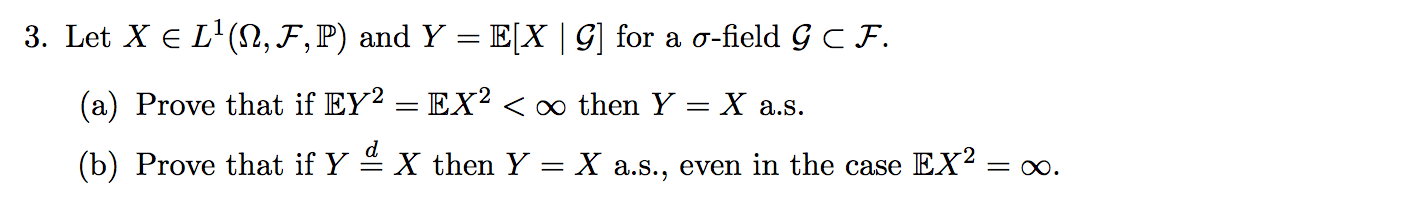
\includegraphics[width=0.7\textwidth]{problim-e9-p3.png}
\end{figure}
\end{question}
\begin{solution} \hfill \\
\textbf{(a)} We compute
\eQnb
\mathbb{E}[(X-Y)^2] &=& \mathbb{E}[X^2] + \mathbb{E}[Y^2] - 2\mathbb{E}[XY] 
\nonumber \\
&=&  \mathbb{E}[X^2] + \mathbb{E}[Y^2] - 2\mathbb{E}[\mathbb{E}[XY|\mathscr{G}]] 
\label{eq:3.1} \\ 
&=& \mathbb{E}[X^2] + \mathbb{E}[Y^2] - 2\mathbb{E}[Y\mathbb{E}[X|\mathscr{G}]] 
\label{eq:3.2} \\
&=& \mathbb{E}[X^2] + \mathbb{E}[Y^2] - 2\mathbb{E}[Y^2] = 0 \nonumber
\eQne
where~\eqref{eq:3.1} holds as the expectation of the conditional expectation of any
$L^1$ random variable is the expectation of the random variable,
and ~\eqref{eq:3.2} holds as $Y$ is $\mathscr{G}$ measurable.
Therefore, $X = Y$ almost surely. 

\bigskip 

\textbf{(b)} We proceed by a standard truncation argument. Let $a > 0$ and $b < 0$.
By conditional Jensen,
\eQb
\mathbb{E}[X \wedge a |\mathscr{G}] &\leq& \mathbb{E}[X|\mathscr{G}] \wedge a
= Y \wedge a \>\>\>\text{almost surely}
\eQe
Since $X = Y$ in distribution, 
\eQb
\mathbb{E}[X \wedge a] = \mathbb{E}[Y \wedge a].
\eQe
Therefore, the above inequality cannot be strict, which implies
\eQb
\mathbb{E}[X \wedge a |\mathscr{G}] = Y \wedge a \>\>\> \text{almost surely}
\eQe
as otherwise by taking the 
expectation both sides, we get a contradiction. Similarly,
\eQnb
\mathbb{E}[(X \wedge a) \vee b |\mathscr{G}] = (Y \wedge a) \vee b 
\>\>\> \text{almost surely} \label{eq:3.b.1}
\eQne
From $X = Y$ in distribution,
\eQb
(X \wedge a) \vee b &=& (Y \wedge a) \vee b \>\>\> \text{in distribution}
\eQe
and hence
\eQb
\mathbb{E}[((X \wedge a) \vee b)^2] &=& \mathbb{E}[((Y \wedge a) \vee b)^2].
\eQe
Therefore, from part (a) and~\eqref{eq:3.b.1},
\eQb
(X \wedge a) \vee b &=& (Y \wedge a) \vee b \>\>\> \text{almost surely}
\eQe
for any $a >0$ and $b < 0$. 
Taking $a \to \infty$ and $b \to -\infty$,
\eQb
X = Y \>\>\> \text{almost surely}.
\eQe

\hfill $\qed$

\end{solution}

\newpage

\begin{question}[4]
\hfill
\begin{figure}[h!]
  \centering
    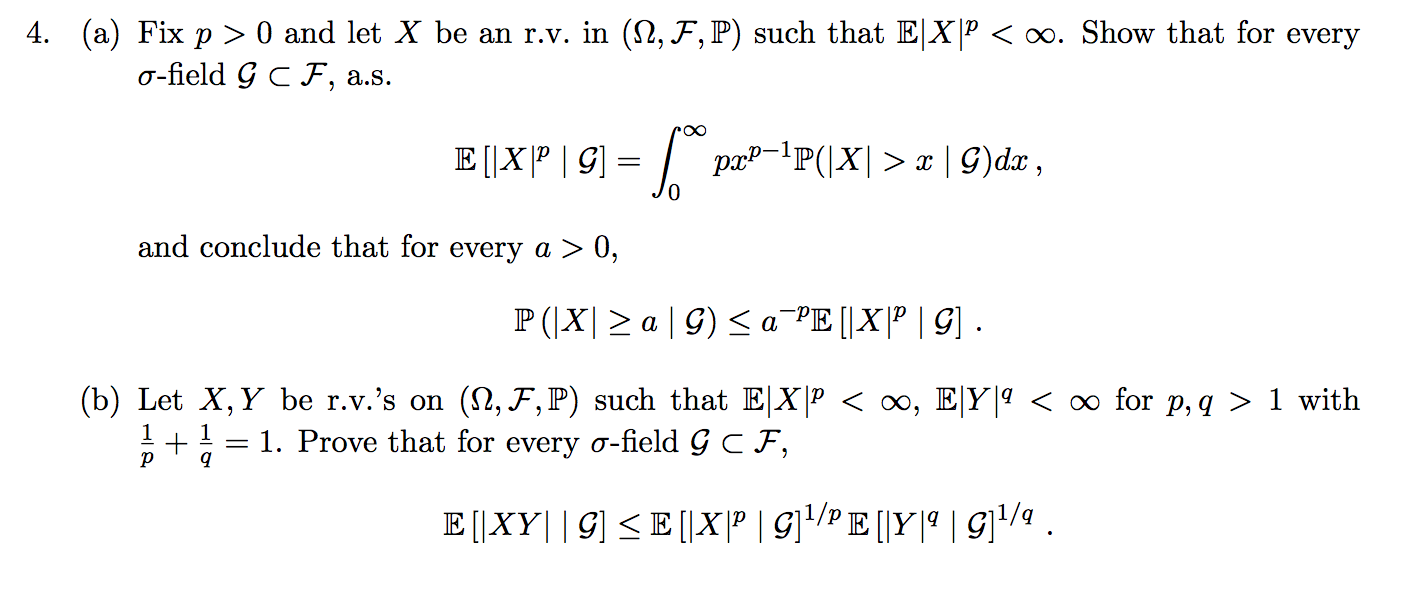
\includegraphics[width=0.7\textwidth]{problim-e9-p4.png}
\end{figure}
\end{question}
\begin{solution} \hfill \\
\textbf{(a)} By Fubini,
\eQb
\mathbb{E}[|X|^p|\mathscr{G}] &=& \int_{\Omega} |x|^p \mathbb{P}(dx| \mathscr{G}) 
= \int_{\Omega} \int_{0}^{\infty} px^{p-1} 1_{\{|X| > x\}} 
dx \mathbb{P}(dx|\mathscr{G}) \\
&=& \int_{0}^{\infty} px^{p-1} 1_{\{|X| > x\}} dx \mathbb{P}(dx|\mathscr{G}) 
= \int_{0}^{\infty} px^{p-1} \mathbb{P}(|X| > x|\mathscr{G}) dx \>\>\> \text{a.s.} 
\eQe
for any $\mathscr{G} \subset \mathscr{F}$. Let $ a> 0$. Then,
\eQb
a^{-p}\mathbb{E}[|X|^p|\mathscr{G}] &=& 
a^{-p}\int_{0}^{a} px^{p-1}\mathbb{P}(|X|>x|\mathscr{G})dx + a^{-p}
\int_{a}^{\infty} px^{p-1} \mathbb{P}(|X| > x|\mathscr{G}) dx \\ 
&\leq& 
a^{-p}\int_{0}^{a} px^{p-1}\mathbb{P}(|X|>x|\mathscr{G})dx + 
\mathbb{P}(|X| = a | \mathscr{G})
= \mathbb{P}(|X| \geq a| \mathscr{G})  \\
\eQe 

\bigskip

\textbf{(b)} Let $A = (\mathbb{E}[|X|^p|\mathscr{G}])^{\frac{1}{p}}$ and
$B = (\mathbb{E}[|Y|^p|\mathscr{G}])^{\frac{1}{p}})$. We compute 
\eQb
\mathbb{E}[|X|^p 1_{\{A = 0\}}] &=& \mathbb{E}[\mathbb{E}[|X|^p 1_{\{A = 0\}}]] \\
&=& \mathbb{E}[1_{\{A = 0\}} \mathbb{E}[|X|^p |\mathscr{G}]] = \mathbb{E}[1_{\{A=0\}}
A^p] = 0  
\eQe  
and hence $|X| = 0$ a.s. on $\{ A = 0 \}$. By the same computation, $|Y| = 0$ a.s.
on $\{B = 0\}$, which implies
\eQb
\mathbb{E}[|XY| |\mathscr{G}] &=& 0 \>\>\> a.s. \>\>\> \text{on} \>\>\> \{A = 0\} \cup
\{B = 0\}.
\eQe
Hence, it suffices to show the inequality on $\Omega_0 = \{A \neq 0\} \cap \{B 
\neq 0\}$. We compute
\eQnb
\mathbb{E}[\dfrac{\mathbb{E}[|XY||\mathscr{G}]}{AB} 1_{G}] 
&=& \mathbb{E}[\dfrac{|X|}{A}1_{G} \dfrac{|Y|}{B} 1_{G}] \nonumber \\
&\leq& (\mathbb{E}[\dfrac{|X|^p}{A^p} 1_G])^{\frac{1}{p}}) 
(\mathbb{E}[\dfrac{|Y|^q}{B^q} 1_{G}])^{\frac{1}{q}} \label{eq:4.b.1} \\
&=& \mathbb{E}[1_G] \nonumber  
\eQne
for any $G \in \mathscr{G}$ where~\eqref{eq:4.b.1} holds by Holder. Therefore,
the inequality holds on $\Omega_0$, so we are done. \hfill $\qed$ 

\end{solution}
\end{document}
